\documentclass{standalone}
\usepackage{tikz}
\usepackage{calc}
\usepackage{pgffor}
\usetikzlibrary{patterns}
\begin{document}
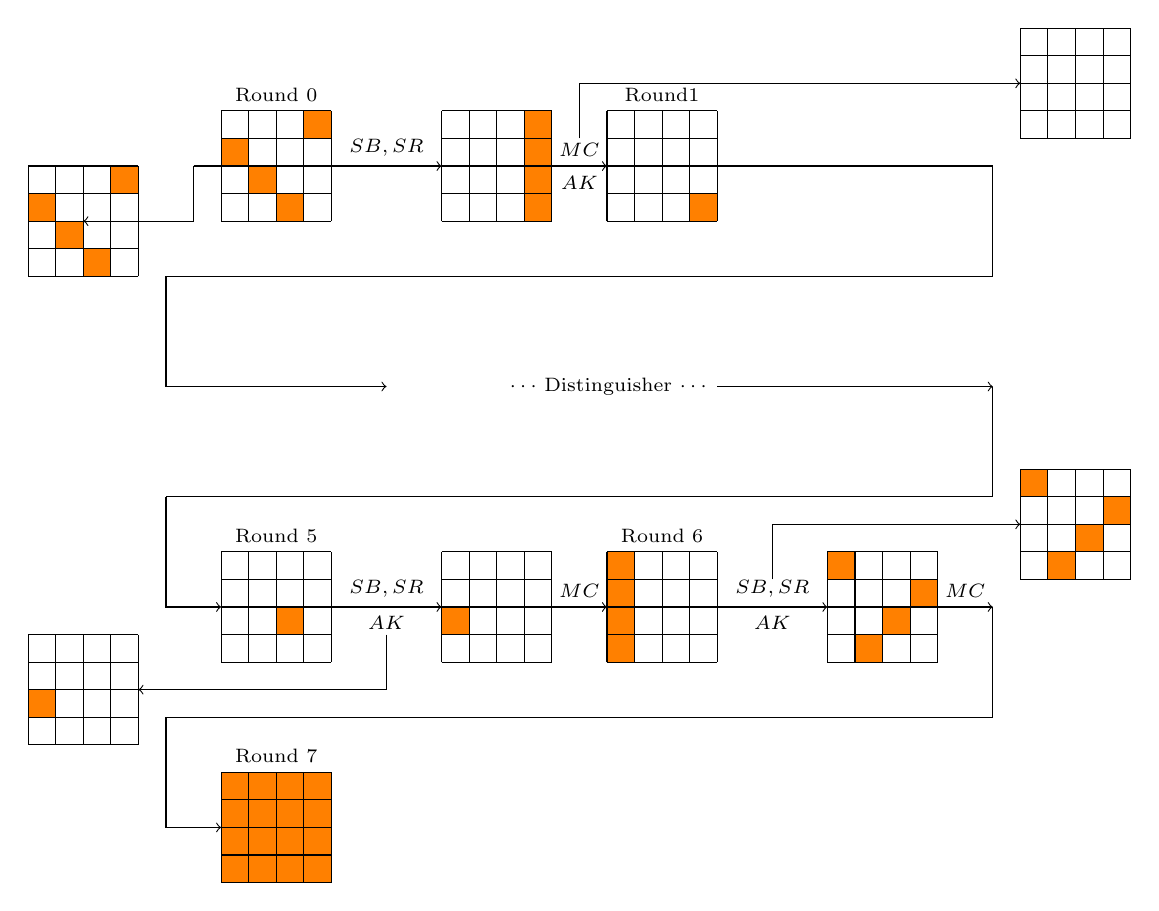
\begin{tikzpicture}[scale=0.35]
\begin{scope}[yshift =0 cm, xshift =0 cm]
\fill[orange](3,3) rectangle +(1,1);
\fill[orange](3,3) rectangle +(1,1);
\fill[orange](11,3) rectangle +(1,1);
\fill[orange](0,2) rectangle +(1,1);
\fill[orange](0,2) rectangle +(1,1);
\fill[orange](11,2) rectangle +(1,1);
\fill[orange](1,1) rectangle +(1,1);
\fill[orange](1,1) rectangle +(1,1);
\fill[orange](11,1) rectangle +(1,1);
\fill[orange](2,0) rectangle +(1,1);
\fill[orange](2,0) rectangle +(1,1);
\fill[orange](11,0) rectangle +(1,1);

\end{scope}
\begin{scope}[yshift =0 cm, xshift =14 cm]
\fill[orange](3,0) rectangle +(1,1);

\end{scope}
\begin{scope}[yshift =0 cm]
\fill[orange](-4,1) rectangle +(1,1);
\fill[orange](-7,0) rectangle +(1,1);
\fill[orange](-6,-1) rectangle +(1,1);
\fill[orange](-5,-2) rectangle +(1,1);
\end{scope}
\begin{scope}[yshift =0 cm]
\foreach \x  in {0,8,14}
\draw[step = 1] (\x,0) grid + (4,4);
\foreach \x in {0}
{\draw[->] (\x+4,2) --node[above]{\scriptsize $SB,SR$}+(4,0);
\draw[->] (\x+12,2) --node[above] {\scriptsize $MC$}+(2,0);
\node[below] at (\x+13,2) {\scriptsize $AK$};
}
\draw (2,4) node[above] {\scriptsize Round 0 };
\draw (16,4) node[above] {\scriptsize Round1};
\draw (18,2)--(28,2);
\draw (28,2) |- ++(-30,-4);
\draw[->] (-2,-2)|-+(8,-4);
\draw[-] (-1,2)--+(1,0);
\draw[->] (-1,2) |-+(-4,-2);
\draw[step = 1] (-7,-2) grid + (4,4);
\draw[->] (13,3) |-+(16,2);
\draw[step = 1] (29,3) grid + (4,4);
\end{scope}
\begin{scope}[yshift =-16 cm, xshift =0 cm]
\draw (2,4) node[above] {\scriptsize Round 5 };
\fill[orange](8,1) rectangle +(1,1);
\fill[orange](2,1) rectangle +(1,1);

\end{scope}
\begin{scope}[yshift =-16 cm]
\fill[orange](-7,-2) rectangle +(1,1);

\end{scope}
\begin{scope}[yshift =-16 cm, xshift =14 cm]
\draw (2,4) node[above] {\scriptsize Round 6 };
\fill[orange](0,3) rectangle +(1,1);
\fill[orange](8,3) rectangle +(1,1);
\fill[orange](0,2) rectangle +(1,1);
\fill[orange](11,2) rectangle +(1,1);
\fill[orange](0,1) rectangle +(1,1);
\fill[orange](10,1) rectangle +(1,1);
\fill[orange](0,0) rectangle +(1,1);
\fill[orange](9,0) rectangle +(1,1);

\end{scope}
\begin{scope}[yshift =-16 cm]
\fill[orange](29,6) rectangle +(1,1);
\fill[orange](32,5) rectangle +(1,1);
\fill[orange](31,4) rectangle +(1,1);
\fill[orange](30,3) rectangle +(1,1);

\end{scope}
\begin{scope}[yshift =-24 cm, xshift =0 cm]
\draw (2,4) node[above] {\scriptsize Round 7 };
\fill[orange](0,3) rectangle +(1,1);
\fill[orange](1,3) rectangle +(1,1);
\fill[orange](2,3) rectangle +(1,1);
\fill[orange](3,3) rectangle +(1,1);
\fill[orange](0,2) rectangle +(1,1);
\fill[orange](1,2) rectangle +(1,1);
\fill[orange](2,2) rectangle +(1,1);
\fill[orange](3,2) rectangle +(1,1);
\fill[orange](0,1) rectangle +(1,1);
\fill[orange](1,1) rectangle +(1,1);
\fill[orange](2,1) rectangle +(1,1);
\fill[orange](3,1) rectangle +(1,1);
\fill[orange](0,0) rectangle +(1,1);
\fill[orange](1,0) rectangle +(1,1);
\fill[orange](2,0) rectangle +(1,1);
\fill[orange](3,0) rectangle +(1,1);

\end{scope}
\begin{scope}[yshift = -8 cm];
\draw[->] (18,2) --node[left=50pt]{\scriptsize $\cdots$ Distinguisher $\cdots$} (28,2);
\draw (28,2) |- ++(-30,-4);
\draw[->] (-2,-2)|-+(2,-4);
\end{scope}
\foreach \z in {2}{
\begin{scope}[yshift = -\z* 8 cm]
\foreach \x  in {0,8,14,22}
\draw[step = 1] (\x,0) grid + (4,4);
\foreach \x in {0,14}
{\draw[->] (\x+4,2) --node[above]{\scriptsize $SB,SR$}+(4,0);
\node[below] at (\x+6,2) {\scriptsize $AK$};
\draw[->] (\x+12,2) --node[above] {\scriptsize $MC$}+(2,0);}
\draw[->] (6,1) |-+(-9,-2);
\draw[step = 1] (-7,-3) grid + (4,4);
\draw[->] (20,3) |-+(9,2);
\draw[step = 1] (29,3) grid + (4,4);
\draw (28,2) |- ++(-30,-4);\draw[->] (-2,-2)|-+(2,-4);
\end{scope}
}
\begin{scope}[yshift =-24 cm]
\foreach \x  in {0}
\draw[step = 1] (\x,0) grid + (4,4);
\end{scope}

\end{tikzpicture}
\end{document}